\subsection{Economics and Investment Markets}

\subsubsection{Valuation and Interest Rates}

\begin{remark} \hlt{Present Value Model}\\
Value of asset is related to expected benefits from holding it.
\begin{equation}
P_t^i = \sum\limits_{s=1}^N \frac{E_t [\widetilde{CF}^i_{t+s}]}{(1+l_{t,s}+\theta_{t,s}+\rho_{t,s}^i)^s} \nonumber
\end{equation}
where $P_t^i$ is value of asset $i$ at time $t$, $N$ is number of CF in life of asset, $\widetilde{CF}^i_{t+s}$ is the uncertain, nominal CF paid $s$ periods in the future, $E_t [\widetilde{CF}]$ is expectation of random variable $\widetilde{CF}$ conditional on information available to investors at time $t$, $l_{t,s}$ is YTM on real default-free investment at time $t$ which pays one unit of currency $s$ periods in the future, $\theta_{t,s}$ is expected inflation rate between $t$ and $t+s$,  $\rho_{t,s}^i$ is risk premium required at time $t$ to pay investor for taking risk in CF of asset $i$ in $s$ periods in the future.\\
The more uncertain the CF, the higher the discount rate (real risk free rate $l$, expected inflation $\theta$, risk premium on uncertainty of CF $\rho$). Value of asset will change if either CF forecasts change, or any of components of discount rate changes. Risk premium varies across asset and investor perception of risk.
\end{remark}

\begin{remark} \hlt{Expectations Impact on Market Valuation}\\
If actual earnings or growth in earnings are above (below) expectations, this may have a positive (negative) effect on firm's value.
\end{remark}

\begin{remark} \hlt{Inter-Temporal Rate of Substitution with Risk-Free Investments}\\
Represents investor trade-off between real consumption now ($u_0$) and in the future ($u_t$).\\
Based on utility theory, the trade-off can then be represented as
\begin{equation}
\widetilde{m}_t = \frac{u_t}{u_0} \nonumber
\end{equation}
Given a quantity of consumption, investors will always prefer current consumption over future consumption, $u_0 > u_t$, hence $\widetilde{m}_t < 1$. If an investor considers an investment in a zero-coupon bond at time $t$ that pays ff one unit of real consumption in $s$ periods, then
\begin{equation}
P_{t,s} = E_t(1 \widetilde{m}_{t,s}) = E_t (\widetilde{m}_{t,s}) \nonumber
\end{equation}
The one-period real risk-free rate of return is then
\begin{equation}
l_{t,1} = \frac{1-P_{t,1}}{P_{t,1}} = \frac{1}{E_t (\widetilde{m}_{t,1})} - 1 \nonumber
\end{equation}
Hence, return is higher for lower current prices. The one-period real risk-free rate is inversely related to inter-temporal rate of substitution.\\
The higher the rate, the more important current consumption is relative to future consumption.\\
Diminishing marginal utility of wealth means investor's marginal utility of consumption decreases as wealth increases. Suggests marginal utility of consumption is higher during periods of scarcity and economic downturn.\\
If investor expects higher income in the future, their expected marginal utility of future consumption decreases relative to current consumption. If investor expects better economic outlook, expectation of higher incomes in future will increase current consumption and reduce savings; vice versa for economic recessions.\\
Investors increase savings rate when expected returns are high or when uncertainty on future income increases.
\end{remark}

\begin{remark} \hlt{Uncertainty and Risk Premiums}\\
Risk aversion of investors can be explained by covariance of investor's inter-temporal marginal rate of substitution and expected returns on savings $\text{cov}_t(\widetilde{P}_{t+1, s-1}, \widetilde{m}_{t,1})$. If underlying cash flows are uncertain, investors demand risk premium for bearing the risk of the uncertainty.  Investor's expected marginal utility of payoff is inversely related level of uncertainty of payoff. Investors experience greater loss of utility for loss in wealth as compared to gain in utility for equivalent gain in wealth (\hlt{Risk Aversion}).\\
Investor's absolute risk aversion declines with wealth, with wealthier investors being less risk-averse. However, marginal utility of holding risky assets declines as investor holds more risky assets in her portfolio. With markets in equilibrium, wealthy and poor investors have same willingness to hold risky assets.
\end{remark}

\begin{remark} \hlt{Risky Premiums on Risky Assets}\\
Considering a risk-free inflation-indexed, zero-coupon bond that investor sell prior to maturity. Uncertainty about price gives rise to risk premium. Price of bond will be lower than expected sale price discounted at real risk-free rate. The risk premium can then be modelled as
\begin{equation}
P_{t,s} = \frac{E_t (\widetilde{P}_{t+1, s_1})}{1 + l_{t, 1}} \text{cov}_t(\widetilde{P}_{t+1, s-1}, \widetilde{m}_{t,1}) \nonumber
\end{equation}
The covariance can be viewed as risk premium.\\
If asset is risky, for risk-averse investors, covariance is negative; when expected future price of asset is high, marginal utility of future consumption relative to current consumption is low. In good economic times, both investor's labour incomes and most risky asset values are high; but with higher future income, marginal utility of future consumption is lower. Resulting negative covariance between marginal utility of consumption and asset prices reduce value of asset for given expected sale price $P_1$. Ceteris paribus, lower current price $P_0$ increases expected return due to positive risk premium.\\
If bond is sold before maturity, the price in one period is unpredictable. For single-period risk-free bond, covariance is zero as there is no uncertainty about terminal value; hence there is no risk premium.
\end{remark}

\begin{remark} \hlt{Default-Free Interest Rates and Economic Growth}\\
If GDP growth is forecasted to be high, utility of consumption in future will be low, and inter-temporal rate of substitution will fall. Investors save less, increasing real interest rates. Hence real interest rates will be positively correlated with real GDP growth rates, which is consistent with existence of high real rates in rapidly growing developing economies. Interest rates are also positively correlated with expected volatility in GDP growth due to higher risk premium.
\end{remark}

\begin{remark} \hlt{Short-Term Interest Rates and the Business Cycle}\\
Short-term nominal zero-coupon government bonds have yields closely related to central bank policy rate. The uncertainty of inflation over very short-term investment horizon ($\sim 3$ months) is negligible.\\
Hence, the nominal interest rate of T-bill is real risk-free rate ($r_f$) and expected inflation ($\pi$):
\begin{equation}
r = r_f + \pi \nonumber
\end{equation}
For longer-term bonds, a risk premium is added for uncertainty related to inflation ($\theta$):
\begin{equation}
r = r_f + \pi + \theta \nonumber
\end{equation}
\end{remark}

\begin{remark} \hlt{Taylor's Rule}\\
Central banks set policy rates to maintain price stability, and achieve maximum sustainable level of employment. Taylor's rule links central bank's policy rate to economic conditions.
\begin{equation}
r_t = l_t + i_t + 0.5(i_t - i_t^{*}) + 0.5(Y_t - Y_t^{*}) \nonumber
\end{equation}
where $r_t$ is policy rate at time $t$, $l_t$ is real short-term interest rates that balance long-term savings and borrowing in economy, $i_t$ is inflation rate, $i_t^{*}$ is target rate of inflation, $Y_t$ and $Y_t^{*}$ are log of actual and potential GDP.\\
Output gap is defined as $(Y_t - Y_t^{*})$, measured in percentage. Positive output gap implies economy is producing more than it can sustain, and is associated with high or rising inflation.
\end{remark}

\begin{remark} \hlt{Yield Curve and the Business Cycle}\\
Policy rule has more significant weight on inflation relative to that of output to stabilise inflation over long term close to target inflation rate. When $i_t \approx i_t^{*}$ and $(Y_t - Y_t^{*})=0$, this is the \hlt{Neutral Policy Rate}.\\
Short-term interest rates and business cycle have interdependent relationship. If short-term interest rates are low for too long, there is risk of credit bubble; if set too high for too long, could lead to recession or depression.\\
Central bank moderate business cycle by modifying policy rate or exaggerating the cycle by not responding optimally to changing economic conditions.
\end{remark}

\begin{remark} \hlt{Yield Curve Slope and the Business Cycle}\\
Yield curve may be used in not just forecasting future rates, but also for future economic activity. Policy rate influences shape of yield curve. Steeply sloping yield curve implies expectation of sharpe increase in interest rates due to high inflation and expected inflation.\\
Steeply inverted yield curve imply expectation of sharply falling inflation and future rates, which may be result of very high nominal policy rates. Inverted curves imply investors expect rates to decrease when current cause of high current inflation are eliminated.\\
Recession is preceded by a flattening or inversion of yield curve. Late stages of business expansion are characterised by peak in inflation and hence relatively high short-term rates. If longer maturity yields reflect lower inflation rates and diminished business credit demand, yield curve tends to flatten or invert. An inverted yield curve often predicts a recession.
\end{remark}

\begin{definition} \hlt{Breakeven Inflation Rate (BEI)}\\
Yield of zero-coupon default-free nominal bond minus zero-coupon default-free real bond of same maturity.\\
Note, for longer maturity bonds, nominal rate is composed of real rate, expected inflation, risk premium for inflation uncertainty. Hence, BEI is composed of expected inflation ($\theta_{t,s}$) and risk premium for uncertainty about actual inflation ($\pi_{t,s}$).
\begin{equation}
\text{BEI} = \theta_{t,s} + \pi_{t,s} \nonumber
\end{equation}
\end{definition}

\begin{remark} \hlt{Credit Cycle and the Business Cycle}\\
Required rate of return for bonds with credit risk includes additional risk premium. The credit risk premium (credit spread) is difference in yield between credit risky bond and default-free bond of same maturity.
\begin{equation}
r_{t,s} = l_{t,s} + \theta_{t,s} + \pi_{t,s} + \gamma_{t,s} \nonumber 
\end{equation}
where $l_{t,s}$ is real short-term interest rate, $\theta_{t,s}$ is expected inflation, $\pi_{t,s}$ is risk premium for uncertainty about actual inflation, $\gamma_{t,s}$ is additional risk premium for credit risk.\\
Credit spreads rise in economic downturns and decrease during expansions. Defaults increase and recovery rates decrease in periods of economic weakness Both effects result in greater credit loss in economic downturns.\\
As credit spreads narrow, credit risky bonds will outperform default-free bonds. Lower rates bonds benefit more than higher rated bonds from narrowing of credit spreads (yields decrease more), vice versa during widening.
\end{remark}

\subsubsection{The Business Cycle}

\begin{remark} \hlt{Industry and Company-Specific Credit Quality}\\
Credit spreads vary across industrial sectors and over time. As credit spreads narrow relative to government bonds, spreads between higher- and lower-rated corporate bond categories narrow; although corporate bonds generally outperform government bonds, lower-rated corporate bonds tend to outperform higher-rated bonds.\\
Types of goods and services by different companies influence credit spreads. Spreads for cyclical companies are more sensitive to fluctuations in economic factors relative to non-cyclical companies.
\end{remark}

\begin{remark} \hlt{Equity and Equity Risk Premium}\\
Discount rate used to value equity securities includes an additional equity risk premium, which is in addition to the risk premium on credit risky bonds as equity is more risky than debt.
\begin{equation}
r_{t,s} = l_{t,s} + \theta_{t,s} + \pi_{t,s} + \gamma_{t,s} + \kappa_{t,s} \nonumber 
\end{equation}
where $\kappa_{t,s}$ is the additional risk premium relative to risky debt for equity.\\
Note, the equity risk premium is $\lambda_{t,s} = \gamma_{t,s} + \kappa_{t,s}$.
\end{remark}

\begin{remark} \hlt{Relationship Between Consumption-Hedging Properties of Equity and Equity Risk Premium}\\
Assets that provide higher payoff in economic downturns are more highly valued due to consumption hedging property of the asset, which reduces the risk premium on the asset.\
Equity prices are generally cyclical, with higher values in economic expansions where marginal utility of consumption is lower. Equity is not the most effective hedging against poor consumption outcomes, hence equity risk premium is positive.
\end{remark}

\begin{figure}[H]
\centering
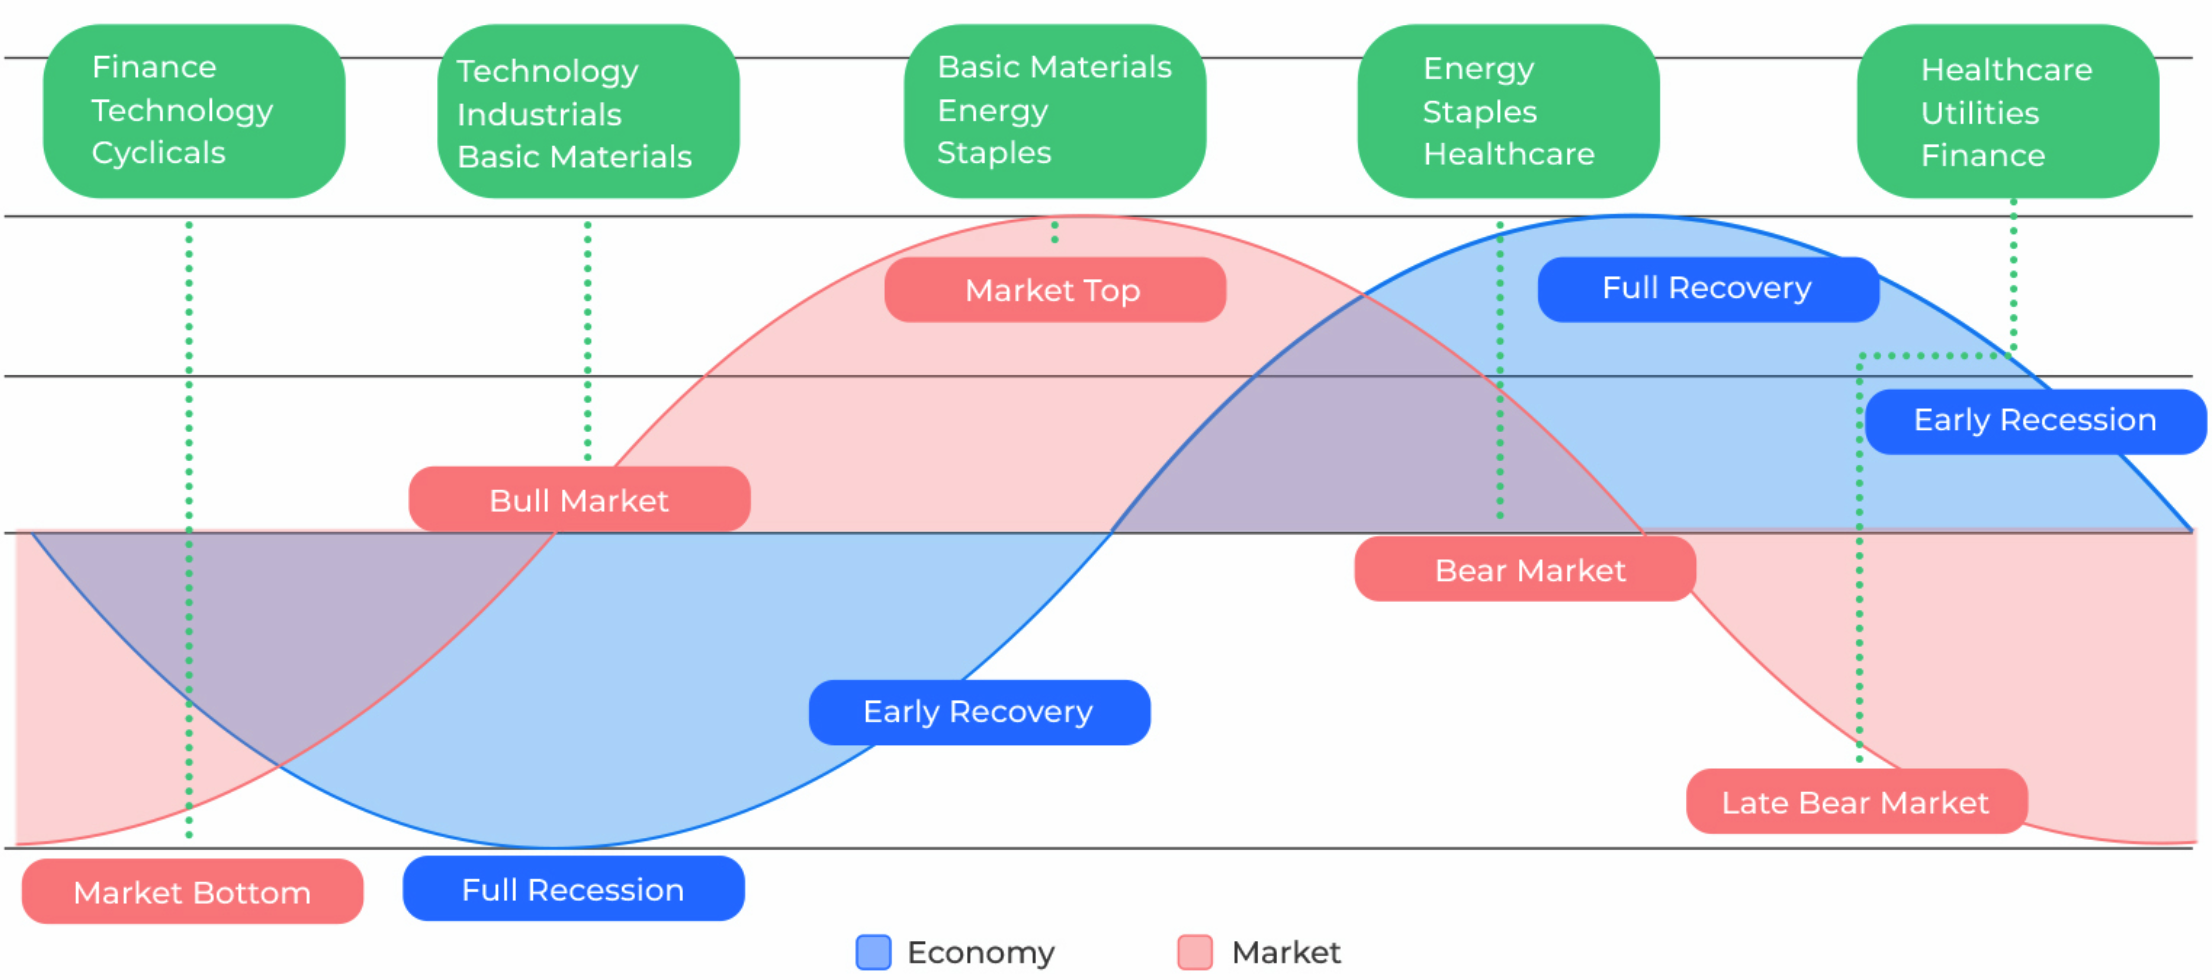
\includegraphics[scale=0.4]{/pm/sectorrotation}
\caption{Sector rotation strategy}
\end{figure}

\begin{remark} \hlt{Earnings Growth Expectations and Business Cycle}\\
Cyclical industries are relatively more sensitive to the phase of business cycle. Companies in these industries have revenues and earnings that rise and fall with the rate of economic growth.\\
Defensive or non-cyclical industries are more immune to fluctuations with more stable earnings.
\end{remark}

\begin{remark} \hlt{Cyclical Effects on Valuation Multiples}\\
Price multiples are positively correlated with expected earnings growth rates, negatively correlated with required returns. Price multiples rise with increases in expected futures earnings growth, and decrease with any components of required rate of return. Hence, equity risk premium declines in economic expansions, vice versa.
\end{remark}

\begin{remark} \hlt{Real Cyclically Adjusted P/E (CAPE) Ratio}\\
Reduces volatility of unadjusted P/E ratios using real (inflation-adjusted) price in numerator, and $10$-year moving average of real (inflation-adjusted) earnings in denominator.
\end{remark}

\begin{remark} \hlt{Real Estate Risk Premiums}\\
For estimation of value of RE, discount rate includes additional risk premium for lack of liquidity.
\begin{equation}
r_{t,s} = l_{t,s} + \theta_{t,s} + \pi_{t,s} + \gamma_{t,s} + \kappa_{t,s} + \phi_{t,s} \nonumber
\end{equation}
where $\kappa_{t,s}$ is risk premium for uncertainty about terminal value of property (similar to equity risk premium), $\phi_{t,s}$ is risk premium for illiquidity.\\
Numerator of present value formula is net rental income, which incorporates expenses incurred.\\
While rental income from commercial properties seems to be steady across business cycles, property values tend to be very cyclical, hence commercial RE values are correlated with those of other asset classes.\\
RE provides poor hedge against poor consumption outcomes, hence risk premium required for investment in commercial RE will be relatively high and often close to risk premium required for equity investments.
\end{remark}